\chapter{The Register File and Bypass Network}

BOOM is a unified, physical register file (PRF) design. The register file holds both the committed and speculative state. The register file also holds both integer and floating point register values. The map tables track which physical register corresponds to which ISA register. 

BOOM uses the Berkeley hardfloat floating point units which use an internal 65-bit operand format (\url{https://github.com/ucb-bar/berkeley-hardfloat}).  Therefore, all physical registers are 65-bits.



\begin{figure}[htb]
	\centering
	\centerline{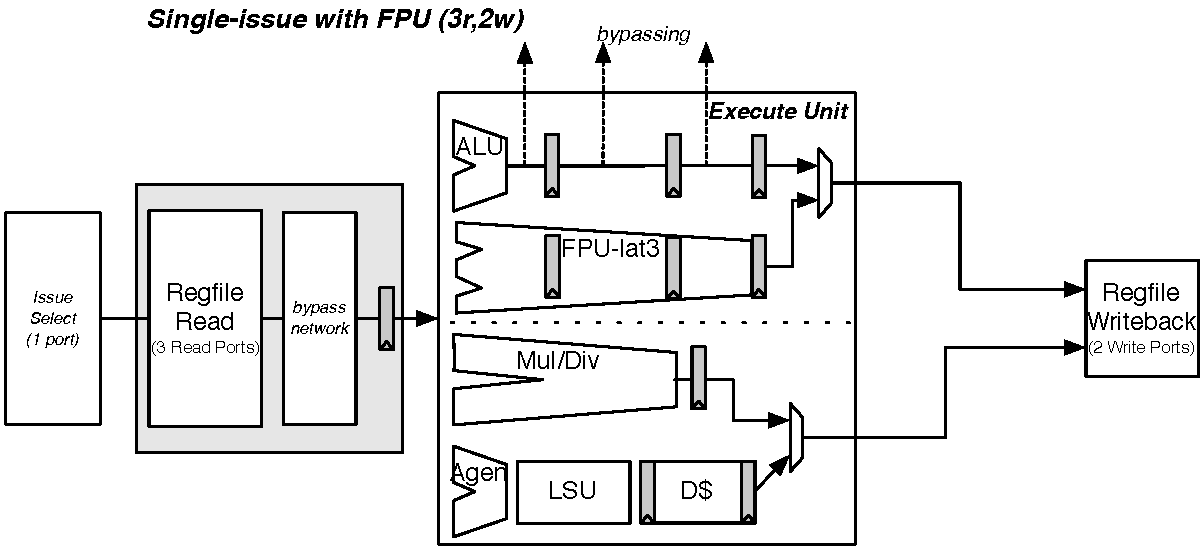
\includegraphics[scale =0.8] {figures/1w-rrd-bypass-pipeline}}
	\caption{ \small An example single-issue pipeline. The register file needs 3 read ports to satisfy FMA operations and 2 write ports to satisfy the variable latency operations without interfering with the fixed latency ALU and FP write-backs. To make scheduling of the write port trivial, the ALU's pipeline is lengthened to match the FPU latency.  The ALU is able to bypass from any of these stages to dependent instructions in the {\em Register Read} stage. }
	\label{fig:1w-rrd-bypass-pipeline}
\end{figure}


\section{Register Read}

The register file statically provisions all of the register read ports required to satisfy all issued instructions. For example, if {\em issue port \#0} corresponds to an integer ALU and {\em issue port \#1} corresponds to a FPU, then the first two register read ports will statically serve the ALU and the next three register read ports will service the FPU for five total read ports. 

\subsection{Dynamic Read Port Scheduling}

Future designs can improve area-efficiency by provisioning fewer register read ports and using dynamically scheduling to arbitrate for them. This is particularly helpful as most instructions need only one operand.  However, it does add extra complexity to the design, which is often manifested as extra pipeline stages to arbitrate and detect structural hazards.  It also requires the ability to kill issued micro-ops and re-issue them from the issue window on a later cycle. 

\section{Bypass Network}

ALU operations can be issued back-to-back by having the write-back values forwarded through the bypass network. Bypassing occurs at the end of the {\em Register Read} stage. 



